\renewcommand{\d}{\mathrm d}
\subject{ESPResSo Tutorial}
\title{The Lattice Boltzmann Method in \ES{}: 
Polymer Diffusion and Electroosmotic Flow
} \author{ Stefan Kesselheim \thanks{\ttfamily 
kessel@icp.uni-stuttgart.de}  \and  Georg Rempfer \thanks{\ttfamily 
georg@icp.uni-stuttgart.de}}
\date{\today}
\publishers{Institute for Computational Physics, Stuttgart University}
\maketitle 
\begin{center}
  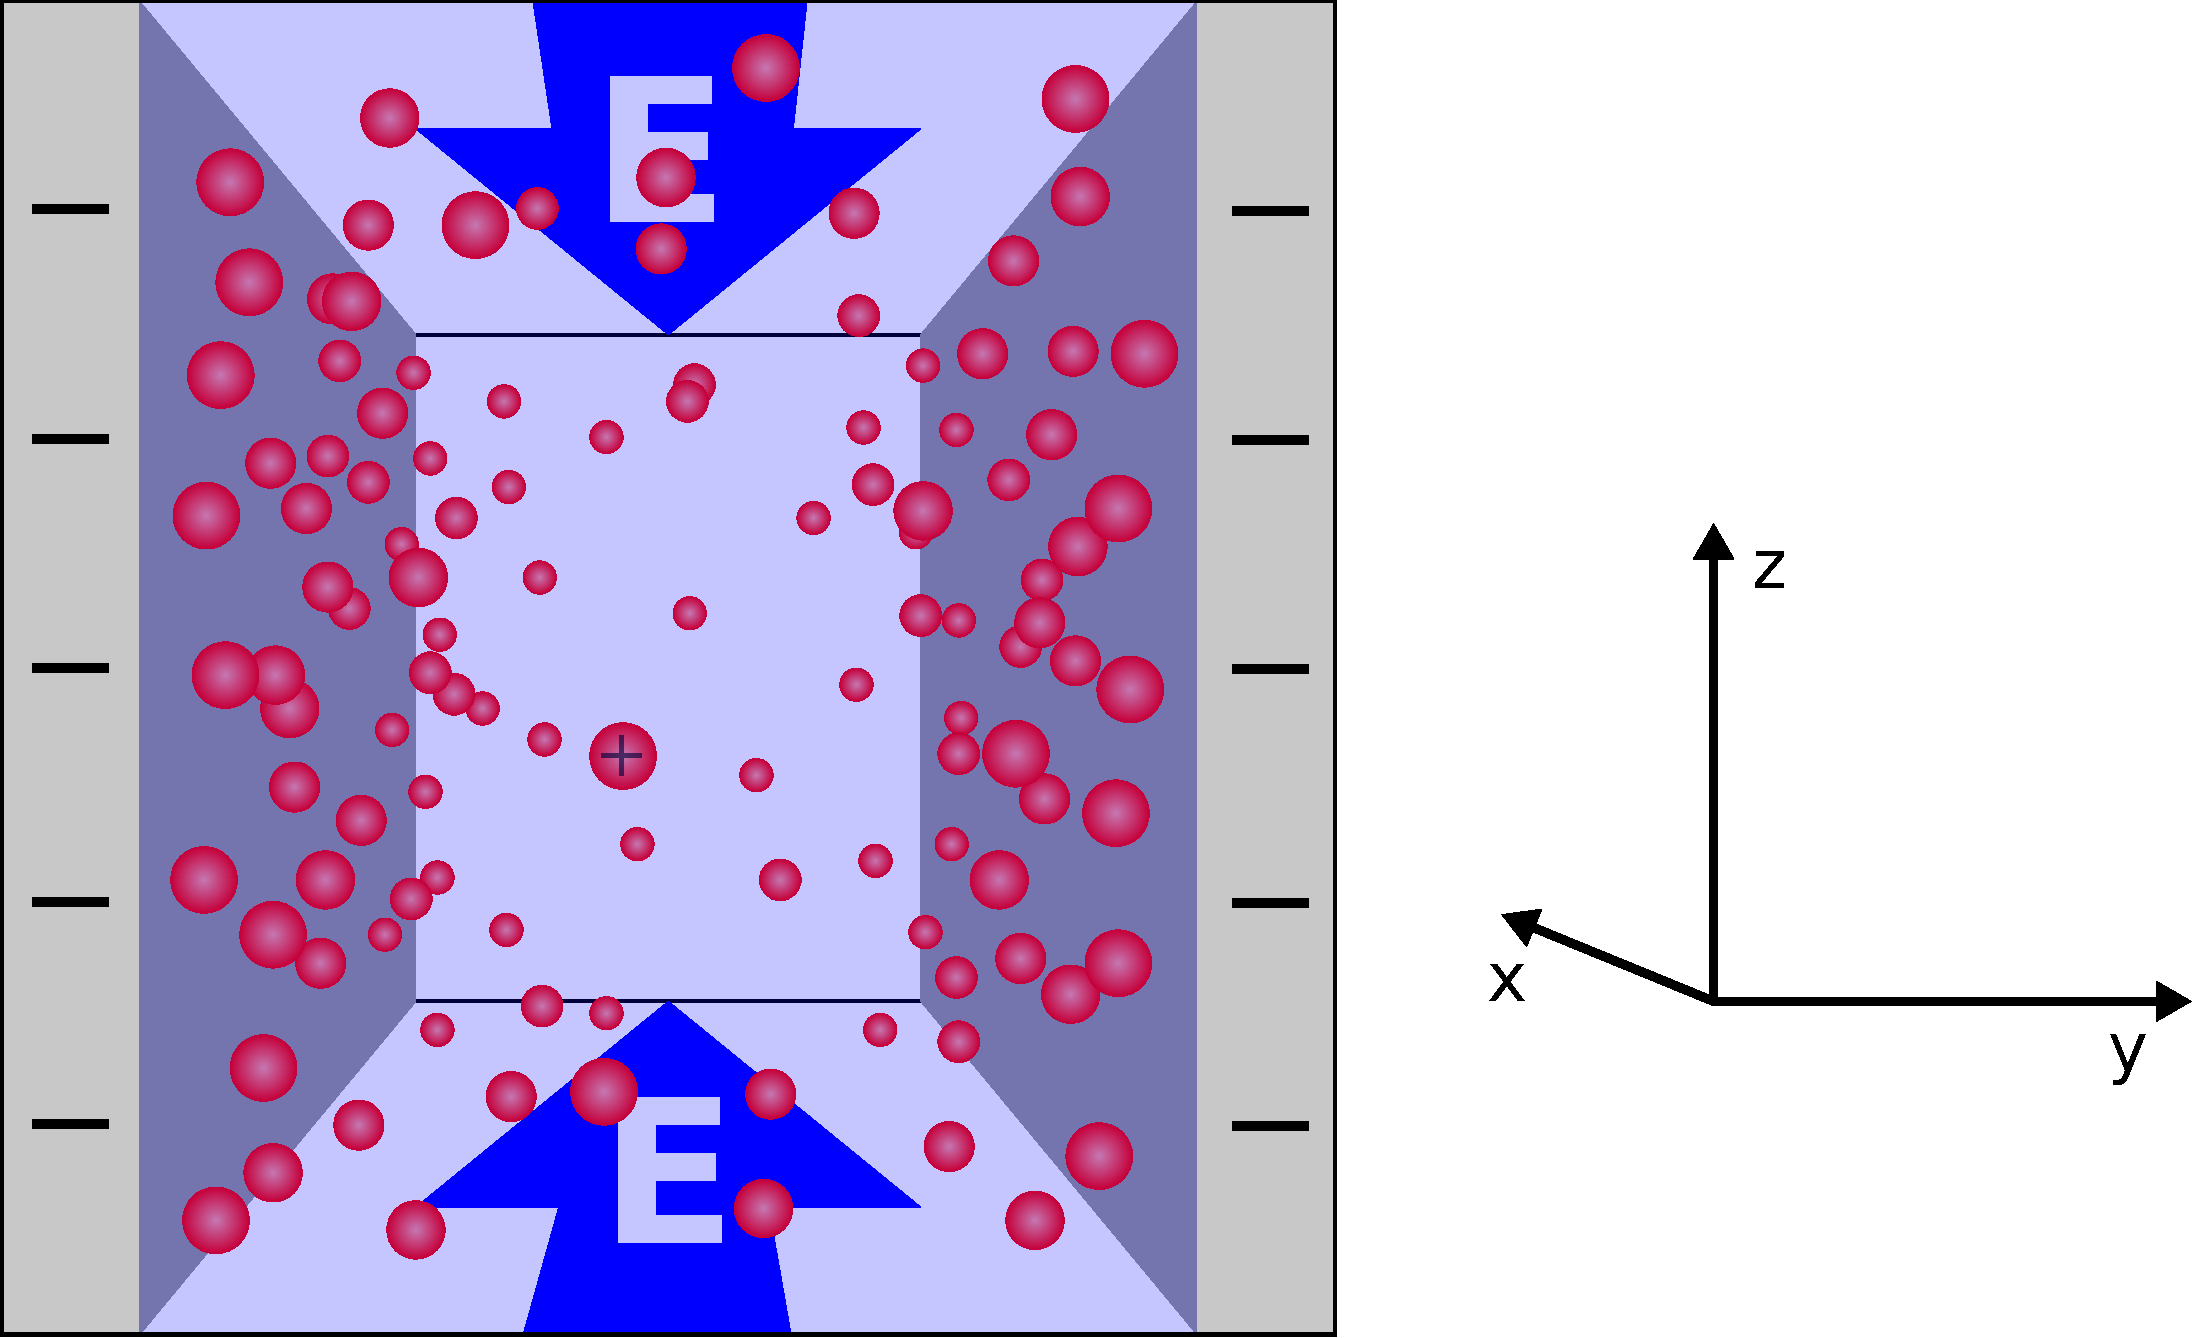
\includegraphics[width=0.5\columnwidth]{../figs/schlitzpore_3d.pdf}
\end{center}
\tableofcontents



 \chapter{Introduction}
In this tutorial, you will learn basics about the 
Lattice Boltzmann Method (LBM) with special focus on the application
on soft matter simulations, or more precisely on how to apply it 
in combination with molecular dynamics to take into account 
hydrodynamic solvent effects without the need to introduce
thousands of solvent particles. 

The LBM -- its theory as well as its applications -- is 
still a very active field of research. After almost 20 years
of development there are many cases in which the LBM has proven
to be fruitful, in other cases the LBM is considered promising,
and in some cases it has not been of any help. We
encourage you to contribute to the scientific discussion 
of the LBM because there is still a lot 
that is unknown or only vaguely known about this fascinating
method. 

\section*{Tutorial Outline}
This tutorial has three main purposes: First, we want to make the start
with the LBM as simple as possible, without leaving out the theoretical
aspects of the LBM.
The second purpose is to show classical examples where the LBM allows 
you to reproduce textbook results.
The third purpose is to show how the LBM can be used with the
\ES{} simulation package. 

\section*{Notes on the \ES{} version you will need}
The LB implementation in \ES{} is currently under major revision
and extension. We (the authors) hope that we could contribute
to an improved usability of this feature of \ES{}. Especially 
the boundary implementation is still very experimental and
not yet published in a release version of \ES{}. Currently 
it is only available from a still unofficial git repository. 
If you want to use it, please contact us.
